\documentclass[a4paper,12pt]{beamer}

\usepackage{préambule}
\usetikzlibrary{arrows.meta}

\newcommand{\myarrow}{-{Latex[length=3mm, width=2mm]}}

\title{Activité : Bonjour !}
\date{}
\author{}

\begin{document}

\begin{frame}
	\maketitle
\end{frame}

\begin{frame}
	\frametitle{Énoncé}

	Des personnes se rencontrent le matin. Elles se disent toutes “bonjour” entre elles. Combien de “bonjour” ont été prononcés si :
	\begin{enumerate}
		\item Il y a 3 personnes ?
		\item Il y a 11 personnes ?
		\item Il y a tous les élèves du collège (939 élèves) ?
		\item Il y a $n$ personnes ?
		\item On suppose qu'il y a 4 personnes. Une nouvelle personne arrive : combien cela rajoute-il de “bonjour” ?
		\item On suppose qu'il y a $n$ personnes. Une nouvelle personne arrive : combien cela rajoute-il de “bonjour” ?
	\end{enumerate}
\end{frame}

\begin{frame}
	\frametitle{Exemple}

	Pour 3 personnes :

	\begin{center}
		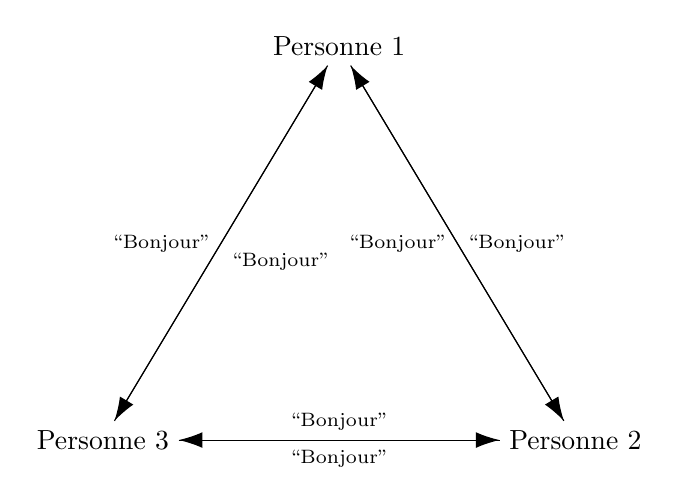
\begin{tikzpicture}[
				mynode/.style={circle,fill=white,anchor=center}]
			\node (P1) at (0,0) {Personne 1};
			\node (P2) at (3,-5) {Personne 2};
			\node (P3) at (-3,-5){Personne 3};

			\newcommand*{\mysize}{\scriptsize}

			\draw[\myarrow] (P1) -- node[right] {\mysize “Bonjour”} (P2);
			\draw[\myarrow] (P2) -- node[left] {\mysize “Bonjour”} (P1);

			\draw[\myarrow] (P1) -- node[below right] {\mysize “Bonjour”} (P3);
			\draw[\myarrow] (P3) -- node[left] {\mysize “Bonjour”} (P1);

			\draw[\myarrow] (P3) -- node[above] {\mysize “Bonjour”} (P2);
			\draw[\myarrow] (P2) -- node[below] {\mysize “Bonjour”} (P3);
		\end{tikzpicture}
	\end{center}

	6 “Bonjour” sont échangés.
\end{frame}

\begin{frame}
	\frametitle{Réponses}

	\begin{enumerate}
		\item 6.
		\item 110.
		\item 880 782.
		\item $n × (n - 1)$.
		\item 8.
		\item $2 × n$.
	\end{enumerate}
\end{frame}

\end{document}